\documentclass[aspectratio=169]{beamer} 

%%% Работа с русским языком
\usepackage{cmap}					% поиск в PDF
\usepackage{mathtext} 				% русские буквы в формулах
\usepackage[T2A]{fontenc}			% кодировка
\usepackage[utf8]{inputenc}			% кодировка исходного текста
\usepackage[english,russian]{babel}	% локализация и переносы

\title{1654. Шифровка (59 pts)}
\author{Дидэ Илья Эдуардович}
\date{1 июля 2022 г.}
\institute{Институт физико-математических наук и информационных технологий БФУ им. И. Канта}

\begin{document}

\frame[plain]{\titlepage} % Титульный слайд

\section{Формулировка задачи}

\begin{frame}
    \frametitle{\insertsection}
    Известно, что Штирлиц шифрует текст следующим образом:
    \newline
        \begin{itemize}
		    \item Убирает все пробелы и знаки препинания.
		    \item Заменяет все подряд идущие одинаковые буквы на одну такую букву.
		    \item Многократно вставляет в произвольное место текста две одинаковых буквы.
		    \newline
	    \end{itemize}
    Попробуйте восстановить текст, каким он был после второго шага. Для этого удалите из текста все пары одинаковых символов, добавленные на третьем шаге.
\end{frame}

\begin{frame}
    \frametitle{\insertsection}
    \begin{block}{Исходные данные}
		В единственной строке записана шифровка Штирлица, состоящая из строчных латинских букв. Длина шифровки не превосходит 200000.
	\end{block}
	\begin{block}{Результат}
		Выведите восстановленный текст.
    \end{block}
    \begin{block}{Пример}
        Исходные данные: wwstdaadierfflitzzz ; Результат: stierlitz
    \end{block}
\end{frame}

\begin{frame}
		\frametitle{Решение задачи}
			\text{\large{\textbf{\textit{Код решения:}}}} \newline	
			(1)\text{\kern 1pc $import\,sys$}\newline
			(2)\text{\kern 1pc $encrypt = sys.stdin.readline()[:-1]$}\newline
			(3)\text{\kern 1pc $decrypt = []$}\newline
			(4)\text{\kern 1pc $for\,x\,in\,encrypt:$}\newline
			(5)\text{\kern 3pc $if\,len(decrypt)\,!=\,0\,and\,decrypt[-1] == x:$}\newline
			(6)\text{\kern 5pc $decrypt.pop()$}\newline
		    (7)\text{\kern 3pc $else:$}\newline
		    (8)\text{\kern 5pc $decrypt.append(x)$}\newline
			(9)\text{\kern 1pc $print("\,".join(str(x)\,for\,x\,in\,decrypt))$}\newline\newline
			\text{\small\textit{Python, версии 3.10}}
	\end{frame}
\begin{frame}
		\frametitle{Ссылки}
		\begin{figure}
			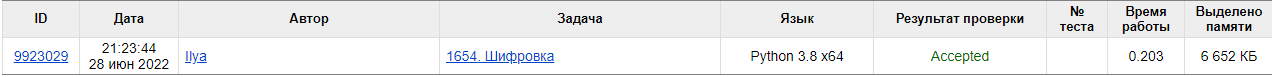
\includegraphics[scale=0.44]{accepted}
			\caption{Проверка на acm.timus.ru}
		\end{figure}
		\begin{itemize}
			\item \href{https://acm.timus.ru/problem.aspx?space=1&num=1654}{Ссылка на задачу}
			\item \href{https://github.com/IlyaDide/Practika}{GitHub-репозиторий}
		\end{itemize}
	\end{frame}

\end{document}
